% Template for Cogsci submission with R Markdown

% Stuff changed from original Markdown PLOS Template
\documentclass[10pt, letterpaper]{article}

\usepackage{cogsci}
\usepackage{pslatex}
\usepackage{float}
\usepackage{caption}

% amsmath package, useful for mathematical formulas
\usepackage{amsmath}

% amssymb package, useful for mathematical symbols
\usepackage{amssymb}

% hyperref package, useful for hyperlinks
\usepackage{hyperref}

% graphicx package, useful for including eps and pdf graphics
% include graphics with the command \includegraphics
\usepackage{graphicx}

% Sweave(-like)
\usepackage{fancyvrb}
\DefineVerbatimEnvironment{Sinput}{Verbatim}{fontshape=sl}
\DefineVerbatimEnvironment{Soutput}{Verbatim}{}
\DefineVerbatimEnvironment{Scode}{Verbatim}{fontshape=sl}
\newenvironment{Schunk}{}{}
\DefineVerbatimEnvironment{Code}{Verbatim}{}
\DefineVerbatimEnvironment{CodeInput}{Verbatim}{fontshape=sl}
\DefineVerbatimEnvironment{CodeOutput}{Verbatim}{}
\newenvironment{CodeChunk}{}{}

% cite package, to clean up citations in the main text. Do not remove.
\usepackage{cite}

\usepackage{color}

% Use doublespacing - comment out for single spacing
%\usepackage{setspace}
%\doublespacing


% % Text layout
% \topmargin 0.0cm
% \oddsidemargin 0.5cm
% \evensidemargin 0.5cm
% \textwidth 16cm
% \textheight 21cm

\title{A new measure of parents' lay theories of parenting and child
development}


\author{{\large \bf Emily Hembacher} \\ \texttt{ehembach@stanford.edu} \\ Department of Psychology \\ Stanford University \And {\large \bf Michael C. Frank} \\ \texttt{mcfrank@stanford.edu} \\ Department of Psychology \\ Stanford University}

\begin{document}

\maketitle

\begin{abstract}
Child development research suggests that parenting practices play an
important role in shaping children's outcomes. For example, children
whose parents engage them in high-quality conversations, and who are
given opportunities for free play, are at an advantage for learning and
later academic outcomes. However, communicating the results of relevant
scientific findings to parents remains a challenge. One possible
moderator of uptake of parenting information is the implicit theories
parents hold with regard to child development and parenting. As a first
step in investigating this possibility, the present work establishes a
new measure of parenting attitudes, and examines whether scores on three
subscales, corresponding to lay theories about rules and respect,
affection and attachment, and early learning, differentially predict
uptake of a popular press article about children's early learning.
Results showed that scores on the early learning subscale, but not the
rules and respect subscale, predicted generalization from the article.

\textbf{Keywords:}
Parenting attitudes; implicit theories
\end{abstract}

Child development research is constantly generating information that can
be brought to bear on best-practices for parenting. For example,
research on children's learning has demonstrated that pedagogy can
improve learning in some contexts and limit it in others, suggesting
that allowing children to play freely and explore is critical for
learning (Bonawitz et al., 2011; Buchsbaum, Gopnik, Griffiths, \&
Shafto, 2011). Likewise, a great deal of research has demonstrated the
importance of engaging young children in elaborative conversations for
language development and future academic success (Hart \& Risley, 1995;
Hoff, 2003; Huttenlocher, Waterfall, Vasilyeva, Vevea, \& Hedges, 2010).
A fundamental challenge we face is how to communicate the results of
such scientific inquiry to a diverse public in a way that maximizes
uptake and improves people's daily and long-term decision making.

One critical parameter that may mediate parenting behavior is parents'
implicit lay theories about child development and parenting. Lay
theories reflect the core beliefs that people hold in different domains,
which may or may not be explicitly articulated, but organize the
processing of new information and decision-making (Dweck \& Leggett,
1988; Ong, Zaki, \& Goodman, 2015). For example, people with an entity
theory of personality tend to interpret people's behaviors as stemming
from fixed personality traits rather than situational factors such as
needs, goals, or emotional states (Dweck, Chiu, \& Hong, 1995). There
are two reasons to focus on parents' lay theories. First, parents' lay
theories might be an important explanatory factor for many of the
behaviors parents engage in with their child. For example, a parent who
believes that building a strong emotional bond with their baby is one of
the most important goals of parenting might have more physical contact
with their child than a parent who does not hold this theory. Secondly,
parents' lay theories may moderate the uptake of new information about
parenting. It is well-established that people more easily encode new
information that is consistent with an existing schema or mental model
they hold (Bransford \& Johnson, 1972). In addition, previous research
has found that interventions on public health beliefs are more
successful when they take into account people's existing belief
structures in the domain (Kumar et al. 2015).

There is some evidence supporting the notion that parents' behaviors are
mediated by implicit lay theories about child development, which vary by
SES and across cultures. For example, cross-cultural studies have found
profound differences in how parents interact with infants; Richman,
Miller \& LeVine (1992) found that mothers in the Gusii community of
Kenya primarily engaged with their children to soothe them when upset,
but did not often speak to them with the goal of engaging or stimulating
them, as did Caucasian parents in the United States. The authors
attribute this to cultural conventions stemming from the belief that
there is no purpose in speaking to infants as they will not understand
what is being said (Richman, Miller \& LeVine, 1992; LeVine, 2004).

There are also important differences in how parents within western
cultures interact with their children. Numerous studies have identified
SES disparities in the amount that parents talk to their children, which
predicts children's language and academic outcomes (Hoff, 2003;
Huttenlocher et al. 2002). In an effort to identify the source of this
disparity, Rowe (2008) discovered that parents' knowledge of child
development (as indexed by their scores on the Knowledge of Infant
Development Inventory; KIDI) predicted their child-directed language,
with more knowledgeable parents speaking to their children more even
when controlling for the amount of speech directed at another adult.
Although this study examined parents' knowledge, and not their lay
theories per se, it provides evidence that people's domain knowledge has
real consequences for their interactions with their children.

There are other examples of parenting beliefs on which parents differ;
Lareau's (2003) theory of ``concerted cultivation'' suggests that higher
SES parents are more likely to view their child's development as a
project that requires a great deal of coordination in the form of
activities and learning experiences, while lower SES parents are more
likely to view their job as keeping their children safe from harm, with
the assumption that they will naturally thrive if given independence.
There have also been hundreds of studies based on Baumrind's (1971)
framework that identifies parents as authoritative, authoritarian, or
permissive, based on their levels of responsiveness and control in their
interactions with their children. Thus, parents' approaches to parenting
appear to vary in predictable ways based on their knowledge and
perceptions about children's learning and development.

Although these previous studies provide preliminary evidence that
parents' beliefs about parenting and child development affect their
parenting behaviors, no previous research has attempted to identify the
underlying theories that might organize their behavior and
decision-making. Previous research has generally relied on observation
of parent-child interactions or self-report of specific activities and
behaviors. To our knowledge there is not an existing measure of parents'
more general attitudes about parenting and child development, which
might drive behavior and predict the uptake of interventions. To address
this gap, the present work establishes a self-report scale that captures
adults' lay theories about child development and parenting. We generated
a questionnaire measuring the degree to which parents endorse three
potential lay theories: a ``rules and respect'' theory, an ``affection
and attachment'' theory, and an ``early learning'' theory. As an initial
test of the external validity of the questionnaire, we conducted an
experiment to investigate whether parents' scores on the theory
subscales would differentially predict their uptake of parenting
information presented via a popular press article about children's early
learning from free play (Gopnik, 2011). We found that higher scores on
the ``early learning'' subscale, but not the ``rules and respect''
subscale, predicted recall and generalization from the target article
(about free play) but not a control article that was unrelated to child
development. Thus, parents' lay theories about parenting and child
development as measured by our questionnaire may be a meaningful factor
in parents' behavior and information uptake.

\section{Scale Construction}\label{scale-construction}

In order to establish a new measure of parenting attitudes, we followed
a structured plan based on psychometric best practices (Clark \& Watson,
1995; Furr, 2010; Simms, 2008). We generated items corresponding to
three hypothesized latent theories about parenting: the Early Learning
theory corresponds to a view of children's early learning that is
consistent with contemporary child development research, and includes
the idea that young children can teach themselves by exploring and
playing. The Affection and Attachment theory captures the notion that
close parent-child relationships are important for development, and
includes the ideas that parents should talk to their children about
their emotions and that children are not spoiled by too much affection.
The Rules and Respect theory corresponds to the idea that parents'
primary role is to enforce rules and encourage behavior control. We
generated items based on a review of the literature on parenting
attitudes, and conducted psychometric analyses on iterative samples of
respondents.

In an initial phase of scale construction, we generated 42 statements
that described attitudes consistent with one of three potential implicit
theories about parenting: Active Learning (12 items; e.g., ``Children
can learn about things like good and bad behavior from an early age''),
Affection and Attachment (10 items; e.g., ``It's important for a baby to
have a strong bond with mom''), and Rules and Respect (20 items; e.g.,
``It is very important that children learn to respect adults, such as
parents and teachers''). These statements were generated based on a
literature review of parenting attitudes and behaviors. The Affection
and Attachment and Rules and Respect subscales are related theoretically
to the Authoritative and Authoritarian dimensions of Baumrind's (1971)
parenting framework, as well as theories of attachment parenting (Jones,
Cassidy, \& Shaver, 2015), but aim to assess beliefs about parenting
rather than overt behaviors. The Early Learning subscale aimed to assess
the extent to which adults believe that it is important to help infants
and toddlers learn through play and conversation.

The initial 42-item scale was administered to 250 adults on Amazon's
Mechanical Turk. Participants used a 7-point Likert scale to report the
degree to which they agreed with each statement from 0 (Do not Agree) to
6 (Strongly Agree). Chronbach's alphas for the three subscales were .86
(Active Learning), .81 (Affection and Attachment), and .74 (Rules and
Respect). We then conducted Exploratory Factor Analysis (EFA) to assess
the dimensionality of the scale. Based on a parallel analysis (Horn,
1965) we retained 5 factors in this initial model. We subsequently
dropped any items that had factor loadings less than .40 on the relevant
factor, as well as any items that had factor loadings greater than .40
onto another factor. Items were also dropped if analyses revealed that
Chronbach's alpha would be increased by dropping the item. Additional
items were dropped such that there were 6 items in each subscale. Some
items were re-worded such that half of the items in each subscale were
negatively worded to avoid response sets (Simms, 2008).

The revised questionnaire was administered to a second group of 250
adults on Amazon's Mechanical Turk. For this sample, Chronbach's alphas
were .76 (Active Learning), .75 (Affection and Attachment), and .69
(Rules and Respect). Because analysis of the previous sample identified
5 factors instead of the hypothesized 3, we again conducted EFA. This
time, the parallel analysis identified 3 factors as predicted. The
subscale items were roughly grouped according to a priori subscales,
although some items from the Affection and Attachment subscale load onto
both the Affection and Attachment and Active Learning subscale factors.

\begin{table}[t]
\centering
\begin{tabular}{lll}
  \hline
Rules and Respect & Affection and Attachment & Early Learning \\ 
  \hline
It is very important that children learn to respect adults, such as parents and teachers. & Parents need to provide safe and loving environments for their children. & Children can learn about things like good and bad behavior from a very early age. \\ 
  It is important for young children to learn to control their impulses (e.g., waiting when told to wait). & Holding and cradling babies is important for forming strong bonds between parent and child. & Young children can teach themselves things by exploring and playing. \\ 
  Children should be taught to be grateful to their parents. & Children should be given comfort and understanding when they are scared or unhappy. & Babies repetitive behaviors (e.g. banging a cup on the table) are a way for them to explore cause and effect. \\ 
  Children should not be punished for breaking small rules. & Parents do not need to talk to their child about his or her emotions. & It is not helpful for adults to explain the reasons for rules to young children because they wont understand. \\ 
  Parents should follow their childrens lead rather than imposing structure in the form of rules. & Children become spoiled if they receive too much attention from parents. & Children dont need to learn about numbers and math until they go to school. \\ 
  Young children should be allowed to make their own decisions, such as what to eat for dinner. & Too much affection can make a child weak. & Reading books to children is not helpful if they have not yet learned to speak. \\ 
   \hline
\end{tabular}
\caption{Parenting Attitudes Scale} 
\end{table}

\section{Experiment 1}\label{experiment-1}

We next conducted an experiment to test whether scores on the three
subscales would predict people's uptake of new information, as an
initial test of the external validity of the scales. For this purpose,
we had participants read two popular press articles: an article arguing
that free play is beneficial to children's learning (Gopnik, 2011), and
an article about the language of smell (Yong, 2015). We operationalized
uptake as accurate recall and generalization of the central message of
the target article, and recall of the control article. We predicted that
if people's subscale scores reflect coherent lay theories, they should
differentially moderate uptake of the two articles. Specifically, we
predicted that scores on the Early Learning subscale would be positively
related to recall and generalization of the target article, but not
recall of the control article. We predicted that scores on the Rules and
Respect subscale would not predict uptake of either article. We excluded
scores on the Affection and Attachment subscale from our analyses, since
they are not orthogonal to scores on the Early Learning subscale.

\subsection{Methods}\label{methods}

\subsubsection{Participants}\label{participants}

Participants were 250 adults recruited from Amazon's Mechanical Turk. Of
these participants, 122 reported having children, 123 reported having no
children, and 5 did not indicate whether or not they had children.

\subsubsection{Procedure}\label{procedure}

Participants first completed the 18-item parenting questionnaire
described above. Participants were then instructed to read two popular
press articles at their own pace. They first read a target article about
children's early learning (``Why Preschool Shouldn't Be Like School,''
Alison Gopnik, Slate, 2011), and then read a control article about the
language of smell (``Why Do Most Languages Have So Few Words For
Smells?'', Ed Yong, The Atlantic, 2015). After reading both articles,
they first answered 5 3afc recall questions about the control article,
and then answered 5 3afc generalization and 5 3afc recall questions
about the target article. The recall questions assessed participants'
memory for specific details of the text, and the generalization
questions assessed participants' ability to generalize from the meaning
of the text to new situations (Fig \#\#) **put examples of questions in
a table?

\begin{CodeChunk}
\begin{CodeOutput}
[1] 48
\end{CodeOutput}
\end{CodeChunk}

\begin{CodeChunk}
\begin{figure*}[!h]

{\centering 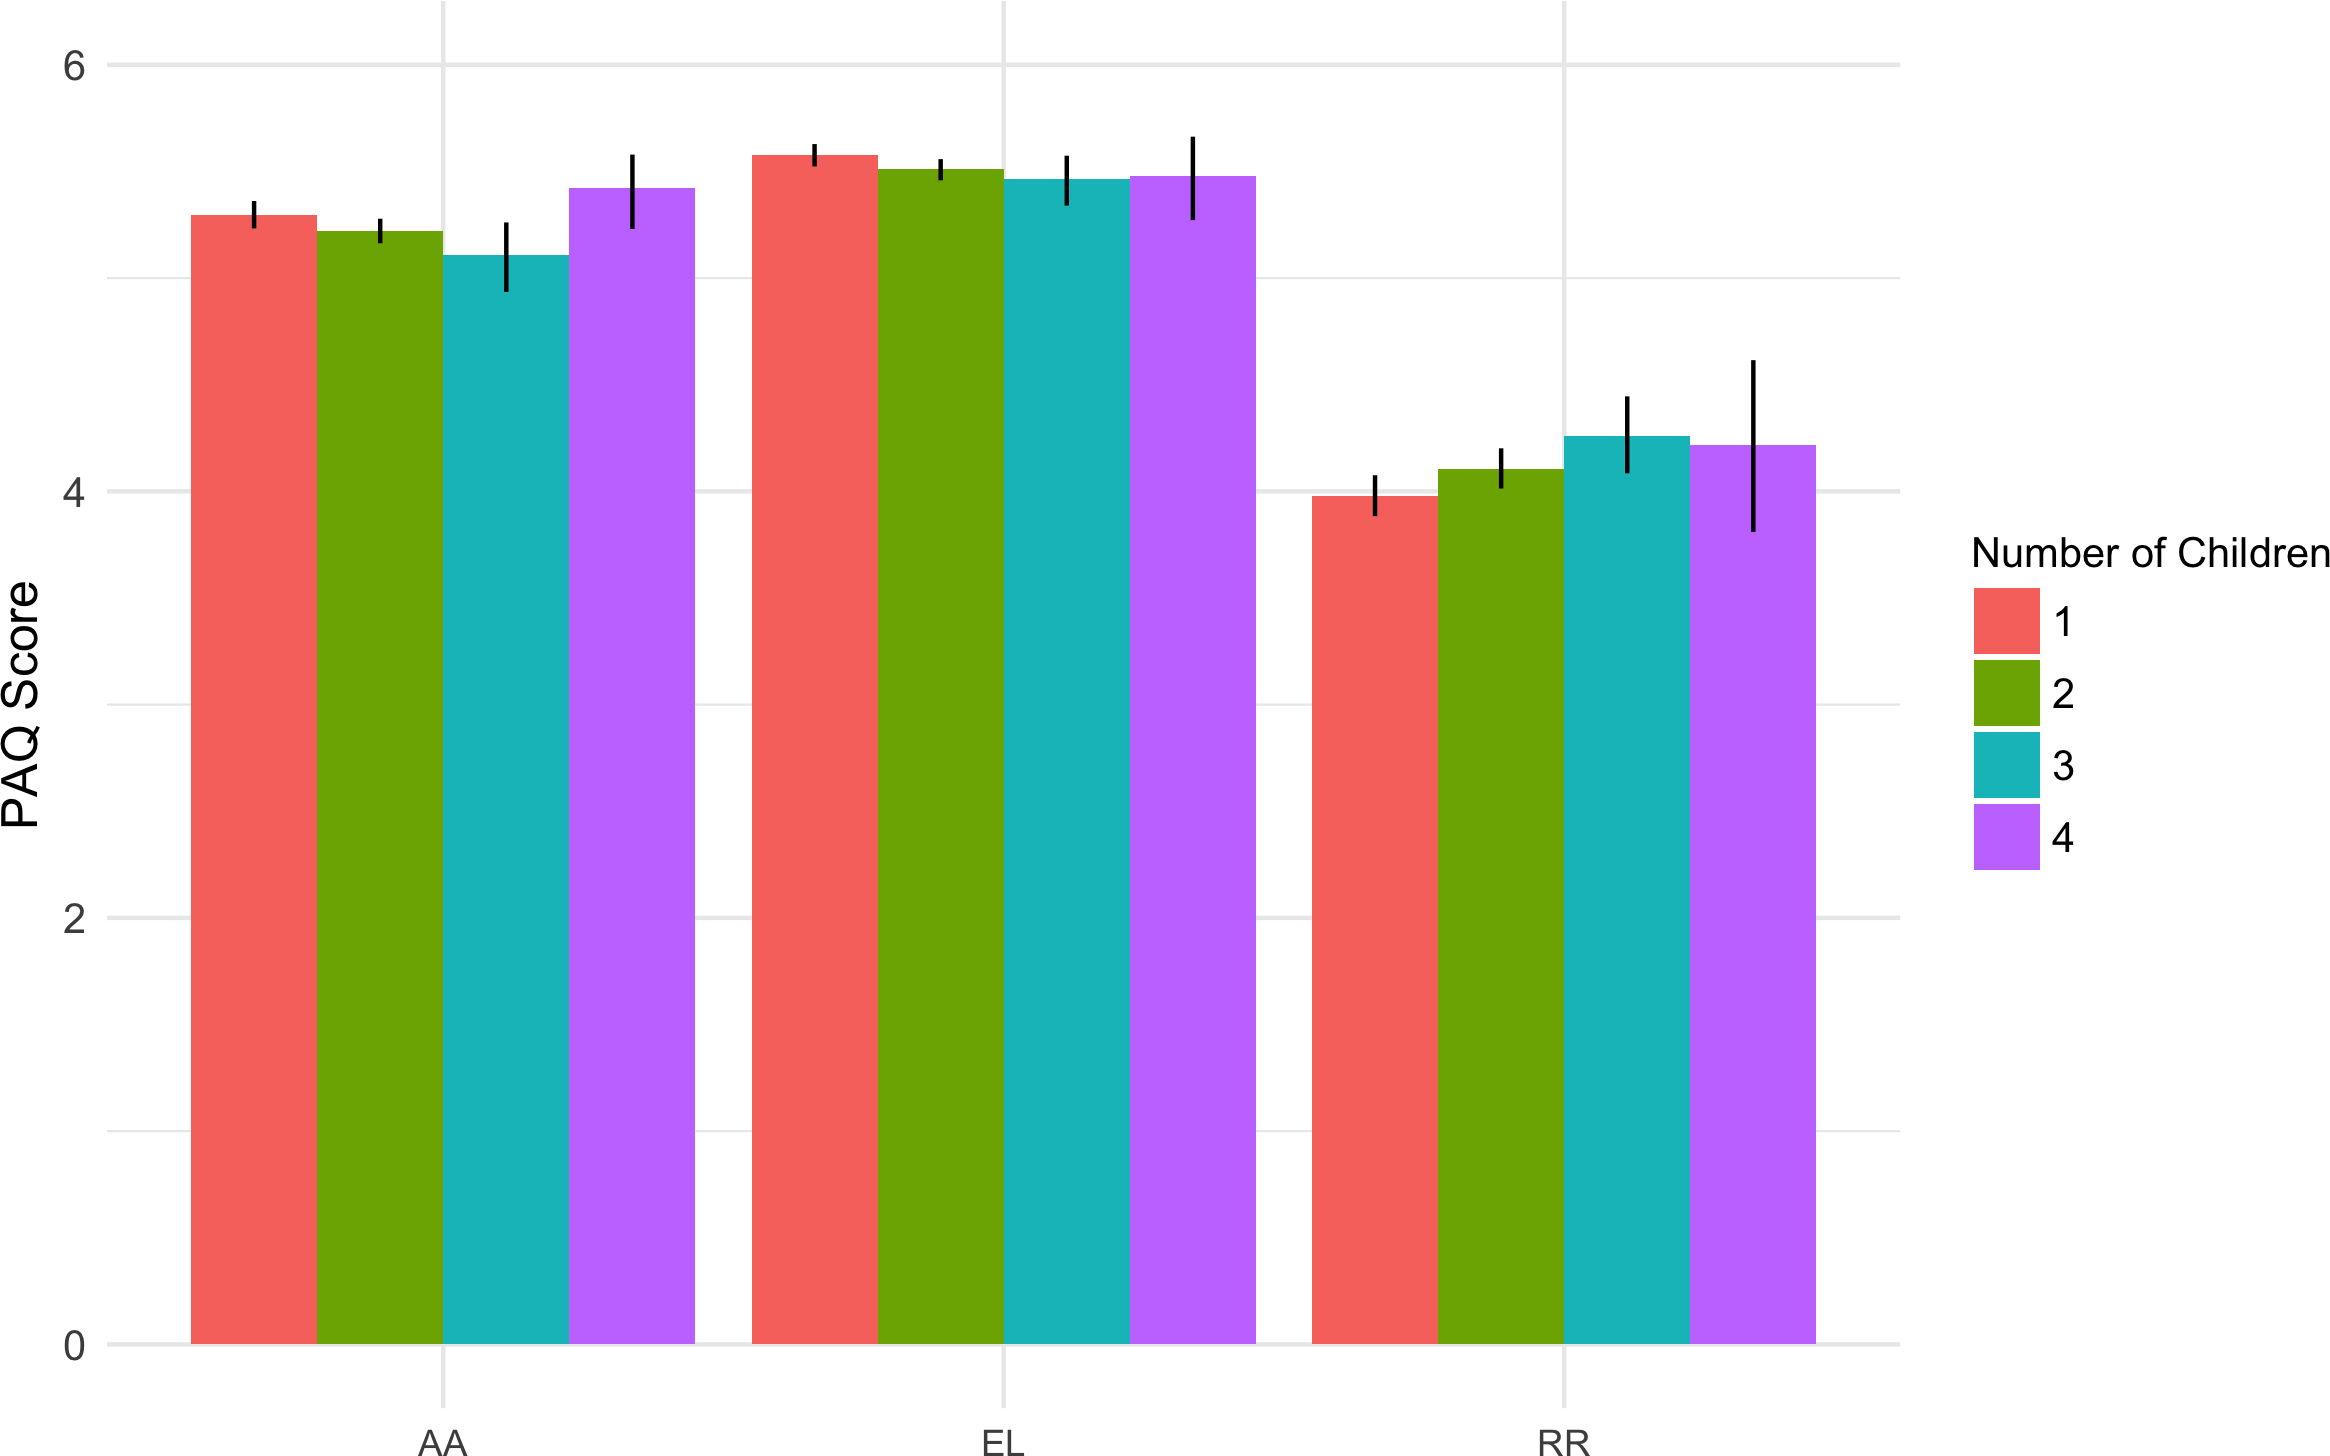
\includegraphics{figs/unnamed-chunk-10-1} 

}

\caption[Relationship between subscale scores and uptake of articles]{Relationship between subscale scores and uptake of articles.}\label{fig:unnamed-chunk-10}
\end{figure*}
\end{CodeChunk}

\subsection{Results}\label{results}

We excluded 48 participants who spent less than 30 seconds reading one
or both of the articles, based on the assumption that they had not had
time to read the whole article. Mean accuracy for the remaining sample
was .67 (SD = .24) for control recall, .83 (SD = .19) for target recall,
and .87 (SD = .22) for target generalization. As we were interested in
whether subscale scores would differentially predict uptake of the
target article compared to the control article, we fit a generalized
linear mixed-effects model with standardized Early Learning and Rules
and Respect subscale scores, as well as interaction terms for the
subscale scores by question type (i.e., control recall vs.~target recall
vs.~target generalization) as fixed effects, and participants and
questions as random effects. Early Learning scores positively predicted
target recall and target generalization, whereas Rules and Respect
scores positively predicted target recall but not target generalization
(Table \#\#).

\subsection{Discussion}\label{discussion}

Understanding the sources of parents' behaviors and decisions with
regard to their parenting is a critical step in improving children's
welfare. There is a large literature outlining the activities and
environments that can make a difference in children's development,
including their language (Hart \& Risley, 1995), executive functioning
(Barker et al., 2014), and conceptual learning (Bonawitz et al., 2011).
However, relevant research findings can sometimes be nuanced and
unintuitive for those outside of academia. Thus, an important challenge
is understanding the lay beliefs parents may have about parenting, and
how they relate to parenting best-practices as identified by
developmental science. Interventions that aim to deliver new information
may be more likely to succeed if they take into account the existing lay
beliefs that parents hold about child development (Kumar et al., 2015).

In the present work, we established a new scale to measure people's
attitudes about parenting and child development in three categories:
Rules and Respect, Affection and Attachment, and Early learning. These
subscales are meant to capture meaningful differences in how people view
child development and the relative importance of different parenting
behaviors. We subjected our new scale to psychometric testing, and found
acceptably high correlations among subscale items, as well as the
predicted factor structure across subscales. In addition, subscale
scores meaningfully predicted uptake of new information about parenting.
Specifically, participants with high scores on the Early Learning
subscale were more likely to generalize the message of the target
article about children's learning to new scenarios, whereas high scores
on the Rules and Respect subscale did not predict generalization of the
article. However, high scores on the Early Learning and Rules and
Respect subscales both predicted recall of the target article. Although
this was not predicted, it is possible that participants who more
strongly endorse the Rules and Respect items are more interested in
child development in general than people who respond more moderately on
those items, which could explain greater recall of the information in
the children's learning article.

In summary, this work provides initial evidence that meaningful
differences in adults' attitudes about child development and parenting
can be assessed by our new scale. Future work should determine whether
subscale scores differentially predict parents observable behaviors with
their children, such as the quality of conversations they engage their
child in, which would provide additional support for our scale.

\section{Acknowledgements}\label{acknowledgements}

This work supported by a gift from Kinedu, Inc. Thanks to members of the
Language and Cognition Lab at Stanford for helpful discussion.

\section{References}\label{references}

\small

\end{document}
